\section{Results}
\subsection{Quantitative results}

We will discuss our quantitative results in terms of the three
measures that we have proposed earlier in the paper.

\subsubsection{Keystrokes Per Character (KSPC)}

\begin{figure}
    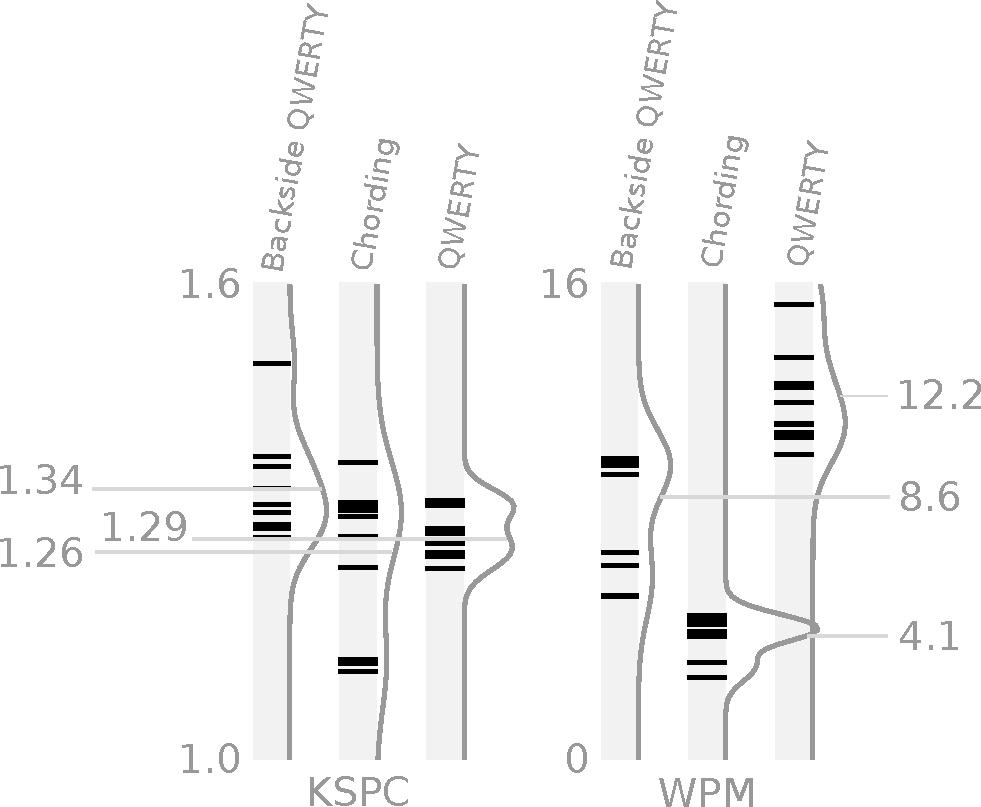
\includegraphics[width=0.5\textwidth]{Figures/kspc_and_wpm.pdf} 
    \caption{Keystrokes-per-character (KSPC) and words-per-minute (WPM) for each mechanism, with means noted. The continous curves represent kernel densities of the population across ranges, 1.0-1.6 for KSPC and 0-16 for WPM. The tiny horizontal bars are scatter plots of individual measurements across the same ranges.}
    \label{fig:kspc_and_wpm}
\end{figure}
From our experiment, it turned out that all the three mechanisms were similar
in terms of KSPC measurements as shown in
Figure~\ref{fig:kspc_and_wpm}.

The Chording mechanism was on an average more accurate than the other two mechanisms, with the Backside QWERTY being the least accurate in terms of average. An ANOVA pointed to a statistically significant main effect of the input technique on the KSPC ($F_{2,33}$ = 4.13, p$<$0.025). A two tailed t-test (for chording versus backside QWERTY) to validate this resulted in a p-value of 0.02, which essentially means that the chording mechanism was significantly more accurate than the backside-QWERTY. 

\subsubsection{Words Per Minute (WPM)}

Our experiment findings suggested that QWERTY was still the fastest
mechanism, followed by backside QWERTY and the slowest was
chording. Statistics on WPM measurements can be found in
Figure~\ref{fig:kspc_and_wpm}. Needless to say that an ANOVA
suggested a main effect of the input technique on the WPM. Pairwise
comparisons suggested that QWERTY was faster than both backside QWERTY
and chording mechanisms. However, it should be noted that the test
sessions were generally around 20-30 minutes, and each user only
interacted with a mechanism once. Therefore, the fact that backside
QWERTY was on a average 3/4th as fast as the QWERTY mechanism was
encouraging. This led us to explore the results qualitatively and also
in terms of speed versus accuracy trade-off.


\subsubsection{Sample tests}

Since the amount of exposure that the users received during the
sessions was limited, it is obvious that lack of experience with the
mechanisms also hampers the speed and accuracy
measurements. Therefore, one of the researchers who was involved in
development of the interface and had reasonable exposure to the
interface went through the test in exactly the same fashion as the
participants. This was done to test the capability of the two new
mechanisms in terms of speed and
accuracy. Table~\ref{tab:StatisticsForTestCorpora} shows the
measurements from the same.  The results are also shown in
Figure~\ref{fig:kspc_and_wpm} for comparison.

\begin{table}
	\centering
		\begin{tabular}{rcc} 
		                         & \color{grey}{WPM}    & \color{grey}{KSPC} \\ 
                   \color{grey}{Chording} & 7.69   & 1.12 \\ 
                   \color{grey}{Backside QWERTY} & 13.231 & 1.152 \\ 
		\end{tabular}
	\caption{Sample Measurements}
	\label{tab:StatisticsForTestCorpora}
\end{table}

We can see from the table and figure that with decent amount of
exposure to the interface, both the accuracy and the speed seem to
improve, suggesting that there are strong learning effects which must
be considered.  These measurements, however, are restricted to an
individual and are highly preliminary. To fully establish our claims,
larger and longer studies would have to be conducted.

\subsubsection{Speed versus Accuracy Trade-off}

\begin{figure}
    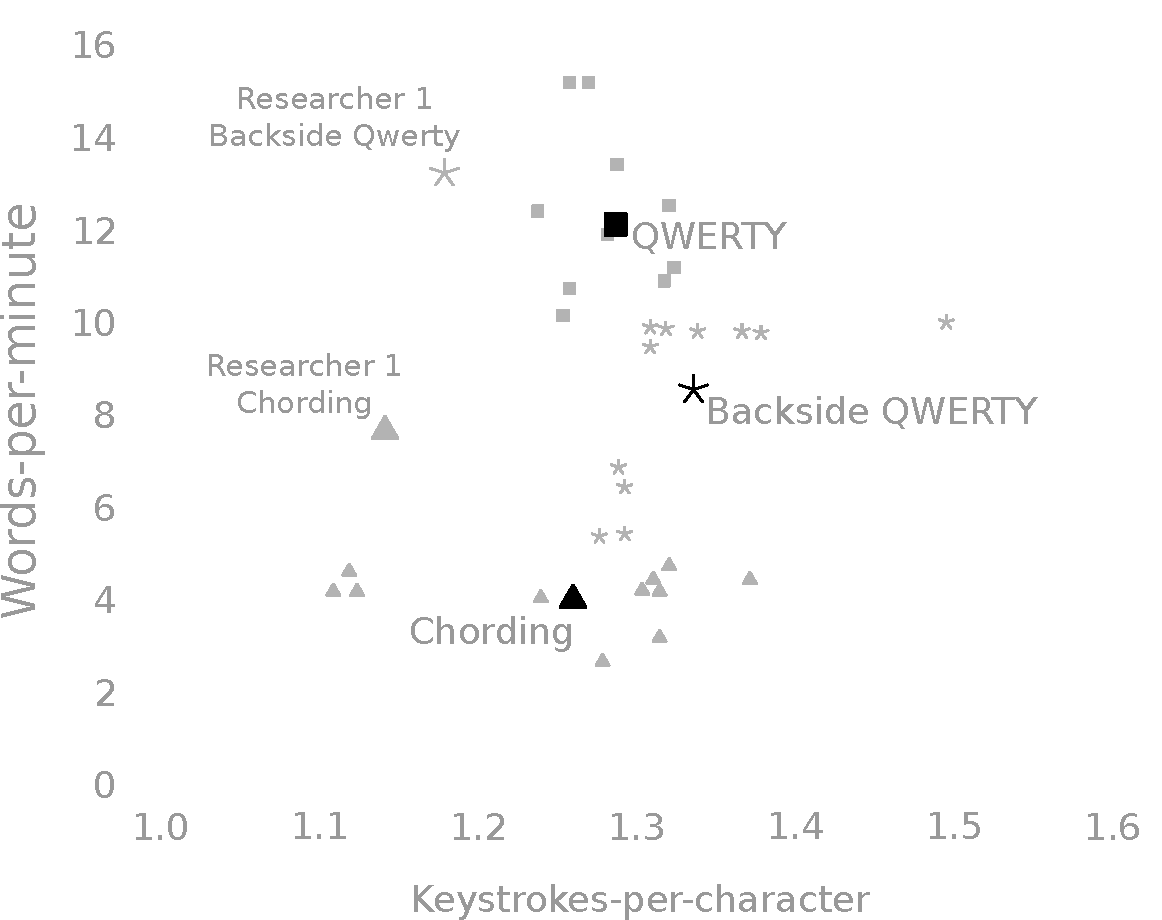
\includegraphics[width=0.5\textwidth]{Figures/kspc_vs_wpm.pdf} 
    \caption{Keystrokes-per-character (KSPC) vs. words-per-minute
      (WPM) for each mechanism.  The large symbols are the mean values
      for each individual mechanism. }
    \label{fig:kspc_vs_wpm}
\end{figure}

In spite of the discussions above, we should acknowledge that none of
these measures can be studied independently, and there was a
possibility that the participants were being more accurate by
sacrificing on speed. However, since speed with a particular input
mechanism is often attributed to the amount of exposure and practice,
we have reasons to believe that the comparison of accuracies is still fair. 

Examining the speed versus accuracy plot for each mechanism suggests
that users reach a limit at which they cannot input data any faster,
despite a sacrifice in accuracy (Figure~\ref{fig:kspc_vs_wpm}).  No
user could break the 10wpm barrier with the Backside QWERTY mechanism,
despite attempts over a wide range of accuracies.  We also had the same observation for the Chording mechanism.

Interestingly, there is a cluster of users who were able to achieve
very high accuracy with the chording mechanism.  This was one of the
primary design goals for the Chording mechanism: to reduce the dependency on precise physical positioning for accurate input.

We hypothesize that the ``speed-limit'' that users reach for the two
novel mechanisms is partly due to the lack of kinesthetic memory
(e.g. muscle memory) operating the keyboard, and unfamiliarity with
the novel chording mechansim.  If this is the case, then concerted
practice should result in faster performance.  Indeed, the results in
Table~\ref{tab:StatisticsForTestCorpora} and
Figure~\ref{fig:kspc_vs_wpm} show just that for at least one user.
Since one user was able to break the ``speed-limit'' with extra
practice, we suspect that the years of extra practice with the QWERTY
mechanism is the primary source of the advantage that QWERTY enjoys.

The high accuracy rates of the Chording mechanism are therefore quite
promising.  In the future, we will need to explicitly examine the
impact of training time on speed and accuracy, and explore methods for
accelerating users' acclimation to the unfamiliar input mechansim.

\subsection{Qualitative results}

As mentioned earlier, we used the NASA task load index to get
subjective ratings on qualitative aspects of the interfaces. In the
following few paragraphs we summarize the trends that were derived
from the ratings that the participants assigned to the backside QWERTY
and chording mechanisms. Figure~\ref{fig:tlx-ratings} presents the
ratings given by the users of all three mechanisms.

\subsubsection{Mental Demand}

An analysis of the mental demand ratings on the NASA-TLX suggested that the participants in the general did not find any mechanism to be more mentally challenging. A one-way ANOVA did not show any main effect of input type on the mental demand ($F_{2.30}$ = 1.74, p$<$0.19). This is encouraging, because it implies that in spite of the slow speed, the participants did not feel that back-of-device interactions were mentally more demanding.

\subsubsection{Physical Demand}

An analysis of the physical demand ratings on the NASA-TLX suggested that the participants in general found the chording mechanism to be the most physically challenging. Looking at the kernel density plots [Figure 7] of the two (backside-QWERTY and chording) revealed that the distribution of population across ratings was very similar in the two interfaces. Therefore, it is reasonably fair to say that the two mechanisms were equally easy or equally hard to use. However, since the averages of all the sets of ratings were around 50 it means that none of the mechanisms were exceptionally hard to use. A one-way ANOVA pointed towards a main effect of input type on the physical demand ($F_{2,30}$ = 3.72, p$<$0.03). However, post-hoc tests (Tukey's HSD, Tukey-Kramer) suggested that there was a significant difference between chording and QWERTY, with p-value of 0.02 (from the t-test between the two). Therefore, from a quantitative standpoint the chording mechanism turned out to be the most physically challenging of the three.

\subsubsection{Temporal Demand}

This metric was important in the sense that we wanted to make sure that the participants did not feel rushed during the task. Our aim was to reproduce the natural experience of entering text, as far as possible. The low average scores (less than 28 for all mechanisms) suggested that the task was not pushing the participants to an extent that they start noticing it. There were constraints that we had specified, but none of them seemed to upset the participants. The fact that there was no time limit to the task, was helpful in this respect. A one-way ANOVA did not point to any significant main effect in terms of the temporal demand, which makes sense given the controlled settings.

\subsubsection{Performance}

The NASA-TLX index ratings for performance suggested that all the interfaces had good performance. The average performance ratings for all the interfaces were below 40 (on 100 point scale). It should be noted that a low rating on this scale means good performance. Also from a quantitative angle, a one-way ANOVA suggested that there was no significant main effect of the type of input technique on the performance ($F_{2,30}$ = 0.4, p$<$0.67). We also observed that there were two users who gave the chording mechanism a higher rating, thereby implying that it did not have good performance. Both these participants had writing speeds that were less than the average. This suggests that these participants were struggling to get accustomed to the device and the mechanism, which might be a possible explanation for the low rating. We also looked at the videos from those sessions, and they corroborated the same claim. 

\subsubsection{Effort}

A one-way ANOVA suggested that there was no significant main effect of the type of input technique on the effort involved ($F_{2,30}$ = 0.87, p$<$0.43). However, studying the kernel density plots (see Figure~\ref{fig:tlx-ratings} more carefully) suggested that the distribution of the opinion on the amount of effort involved in working with the backside-QWERTY was less evenly distributed. However, for the chording it was almost evenly distributed around the average rating. The videos suggested that some of such cases were because the backside-QWERTY did not allow for change in size of the keyboard, people who had fingers longer or shorter than average finger sizes had a harder time with the mechanism as opposed to other. The chording mechanism on the other hand, did allow for such changes and therefore possibly got an even distribution of ratings.

\begin{figure*}
    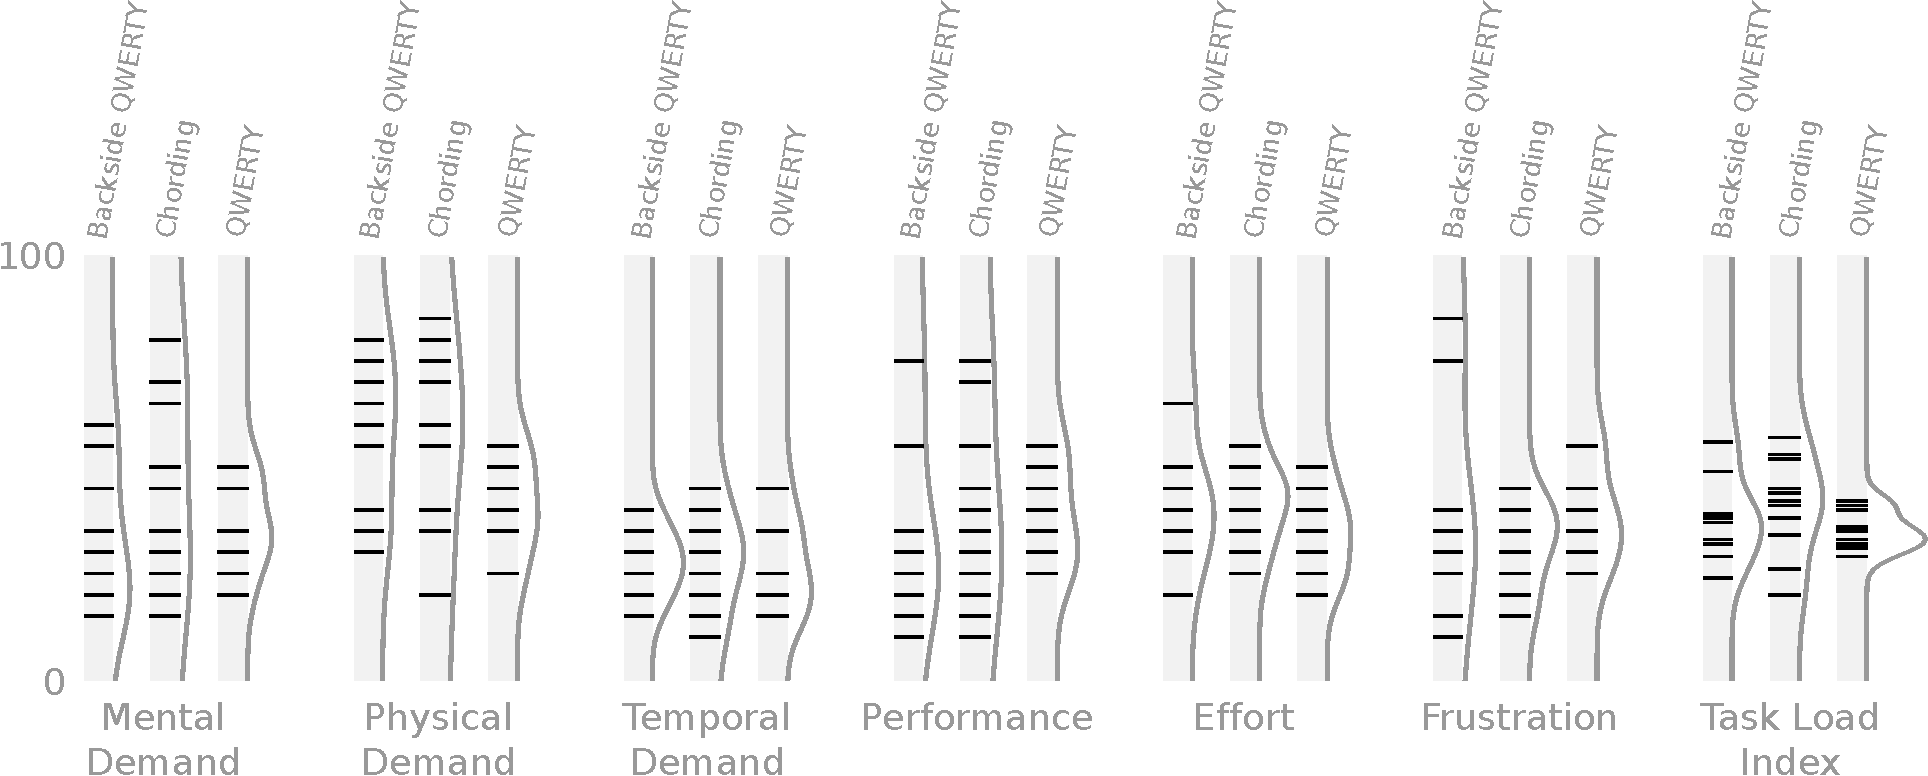
\includegraphics[width=\textwidth]{Figures/hash_and_densities_index.pdf} 
    \caption{NASA-TLX rating for all three input mechanisms}
    \label{fig:tlx-ratings}
\end{figure*}


\subsubsection{Frustration}

A one-way ANOVA suggested that there was no significant main effect of the type of input technique on the frustration ($F_{2,30}$ = 0.36, p$<$0.7). The ratings suggested that on an average users were satisfied with the mechanisms. The frustration levels/ratings were restricted to the lower half of the scale for chording, however only two users reported higher levels of frustration with the backside-QWERTY. When we cross-checked this with our video logs, it turned out that both of these users had issues with getting accustomed to the mechanisms primarily because of finger sizes, as pointed out in the last section. This in turn resulted in the observed frustration on the NASA-TLX.

\subsubsection{Mean Weighted Scores}
After the individual analysis of the ratings, we used the standardized methods to calculate the effective weighted task load ratings, as specified by NASA. Right after filling up the survey, the participants were also asked to compare metrics against each other. Since there were 6 metrics (Mental, Physical, Temporal, Performance, Effort, Frustration), there were $C_{2}^{6}$ possible combinations, and 15 questions in total. After receiving all the responses from the
participants, we found that on an average effective weights for Mental Demand, Physical Demand, Temporal Demand, Performance, Effort, Frustration were 4, 3, 3, 1, 2, 2 respectively. In simple words, a higher weight means that particular dimension or metric has larger effect towards the load of the task and should be given more weightage as opposed to others. Initially we thought that interactions with backside-QWERTY and chording mechanisms were intrinsically different tasks, and therefore the weights should not be treated as the same. However, the average weights that were calculated for the two mechanisms turned out to be the same. This is understandable from a viewpoint that both the tasks were actually text entry tasks with same corpus, and same kind of input method. Therefore, the value that the participants were attaching to each metric didn't change. This is also correct in view of previous research on the NASA-TLX \todo{cite TLX paper}.

It is apparent from the discussion above, but to clarify again, a low weighted score on the NASA-TLX means that the overall task load was low and the experience was pleasant. The backside-QWERTY obtained a weighted score of 37 on an average, and the chording mechanism got an average score of 41. The average score for QWERTY was 35. A one-way ANOVA suggested that there was no significant main effect of the type of input technique on the perceived effective workload ($F_{2,30}$ = 0.59, p$<$0.56). This result is very encouraging and exciting as it implies that after the experiment, in spite of the slower speed, the users did not perceive the back-of-device input techniques as harder to perform. 

\subsection{Design guidelines}

After a qualitative and quantitative analysis of our results, we also did a high-level analysis of our design choices and cross-checked them against the videos. As a result of this, we came up with some major design takeaways from this piece of research. Therefore, in this section we propose some design guidelines for future efforts that look into text input by utilizing a backside touch input device. 

\subsubsection{Movement minimization}

During the study we realized that the amount of movement involved in selecting a particular character determines the speed that users would achieve with the mechanism. The post-experiment analysis of usability test videos corroborated this claim. Once we reduced the size of the keys and magnified the movement of fingers, the users could cover larger distances with smaller shifts in position. We also realized that users are able to control the finger position with very high accuracy because their finger positions were anchored to the side of the device, and therefore these optimizations help them enter text at higher speeds.

\subsubsection{Multiple finger sizes}

There can be a lot of variation in finger sizes, amongst users. We accounted for this in the chording mechanism, by having settings that the user could select, if they had fingers larger or shorter than the average. This was critical for chording mechanism as the users were trying to form chords at specific locations. For backside-QWERTY, we did not make this optimization because users were not trying to position multiple fingers at the same time, and also because in that case we had tried to optimize between finger movement and key sizes.

\subsubsection{Reducing dimensions of movement}

This one is only true for the chording mechanism, but it turned out from the experiment that a good way to maximize on accuracy is to reduce the number of dimensions of movement. Traditionally, with a soft-QWERTY users tend to position themselves in both, x and y coordinate. In the chording mechanism, the y direction was being controlled by the number of fingers, and therefore the movement was just restricted to the x direction.

\subsubsection{Visual search vs Recall}

After the usability testing we also realized that without the tactile feedback of a keyboard, users tend to do a visual search to find characters instead of recalling from their previous experiences with QWERTY mechanisms. As long as the positions of characters follow a pattern, either pre-existing
(like QWERTY) or familiar (alphabetic), users will be able to accustom themselves in a few interactions.

\subsubsection{Touch Cursors}

Both our mechanisms involved showing finger positions on the screen and we had to this in a way that we don't hide any information or don't cause a loss of perception. We achieved this by doing a number of things. We made the touch cursors transluscent, so that we don't occlude any information. We also kept the size of the cursor smaller than the size of an individual key so that they are easier to position and don't end up selecting multiple keys at the same time.
